\begin{frame}{Valorisation des archives de Jean-Martin Charcot}
	\vspace{-3ex}
	\begin{table}[h]
		\begin{tabular}{|c|}
			\hline
			\fontsize{9}{10}\selectfont \textit{Dans les petits papiers de Charcot : de l'expérimentation aux prémisses de la neurologie moderne\footnote{\url{https://theses.fr/s382733}}} \\ \hline
		\end{tabular}
	\end{table}
	\bigskip
	\begin{columns}
		\column{0.40\textwidth}
		Thèse en cours \\
		\footnotesize{initiative \textsc{OPUS}}%
		\setcounter{footnote}{1}% Force the counter to "b"
		\footnote{\url{https://institut-opus.sorbonne-universite.fr/node/478}}\\
		\begin{itemize}
			\footnotesize
			\item dir. : Prof. D\textsuperscript{r} Glenn ROE
			\item co-enc. : D\textsuperscript{r} Motasem ALRAHABI
		\end{itemize}
		
		\column{0.48\textwidth}
		\begin{figure}
			\centering
			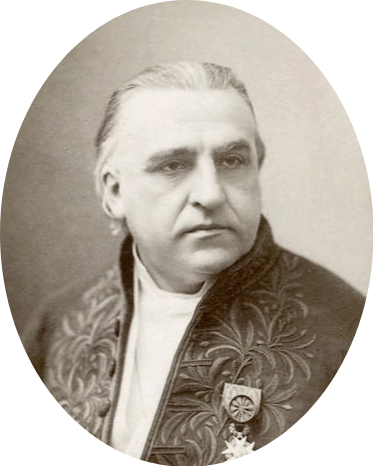
\includegraphics[width=.25\textwidth]{pic/Jean-Martin_Charcot-modified.png}
			\caption{J.-M. Charcot (1825-1893), \href{https://fr.wikipedia.org/wiki/Jean-Martin_Charcot\#/media/Fichier:Jean-Martin\_Charcot.jpg}\\
				{Wikipédia}.}
		\end{figure}
					\begin{itemize}
			\small
			\item père de la neurologie moderne
			\item hystérie, \og{}Parkinson\fg{}, \textsc{SLA}$\dots$
			\item Freud, de la Tourette, Babinski$\dots$
			%			\item Fonds Charcot sur SorbonNum\footnote{\url{https://patrimoine.sorbonne-universite.fr}}
		\end{itemize}
	\end{columns}

\end{frame}
